% =============================================================================
% slides_v2_handout.tex
% Beamer handout mode driver for slides_v2.tex
% Suppresses overlays and pauses; prints 2 slides per A4 page
%
% Compile: xelatex slides_v2_handout → biber slides_v2_handout → xelatex ×2
% =============================================================================
%
% How it works:
%   \PassOptionsToClass{handout}{beamer} injects the [handout] option before
%   \documentclass{beamer} is called inside slides_v2.tex, suppressing all
%   overlay specifications (\pause, \only<2->, etc.).
%
%   The pgfpages layout is configured via \AtEndPreamble to ensure it runs
%   after all packages in slides_v2.tex have loaded.
%
% =============================================================================

\PassOptionsToClass{handout}{beamer}

% Inject pgfpages 2-on-1 layout after the preamble of slides_v2 loads
\RequirePackage{etoolbox}
\AtEndPreamble{%
  \RequirePackage{pgfpages}%
  \pgfpagesuselayout{2 on 1}[a4paper,border shrink=5mm]%
}

% ============================================================================
% slides_v2.tex
% Beamer deck for: Liquidity, Activism Disclosure, and Takeover Premia
% Version 2: Restructured 17 main + 8 backup slides
% ============================================================================
\documentclass[aspectratio=169,11pt]{beamer}

\usetheme{ucl}
\useoutertheme[small]{ucltitlebanner}

% Title page: use plain black text (no banner-colored title box)
\setbeamercolor{title}{fg=black,bg=}
\setbeamerfont{frametitle}{series=\bfseries}

%packages
\usepackage{amsmath,amssymb,amsfonts}
\usepackage{booktabs}
\usepackage{graphicx}
\usepackage{array}
\usepackage{tabularx}
\usepackage{tikz}
\usetikzlibrary{arrows.meta,positioning,shapes.geometric,calc,decorations.pathreplacing}
\usepackage{csquotes}

\usepackage[backend=biber,style=authoryear,natbib=true,maxcitenames=2,maxbibnames=99]{biblatex}
\addbibresource{slides.bib}

%notation (match draft.tex)
\newcommand{\E}{\mathbb{E}}
\newcommand{\PP}{\mathbb{P}}
\newcommand{\1}{\mathbf{1}}
\newcommand{\Var}{\mathrm{Var}}
\newcommand{\Cov}{\mathrm{Cov}}
\newcommand{\R}{\mathbb{R}}

%color coding for notation
\usepackage{xcolor}
\newcommand{\choice}[1]{\textcolor{blue}{#1}}
\newcommand{\obs}[1]{\textcolor{red!70!black}{#1}}
\newcommand{\outcome}[1]{\textcolor{green!50!black}{#1}}

%beamer cosmetics
\setbeamertemplate{navigation symbols}{}
\setbeamertemplate{footline}[author title date]

%blocks: high-contrast callouts (no dark fill)
\setbeamercolor{block title}{fg=brightblue,bg=}
\setbeamercolor{block body}{fg=black,bg=}
\setbeamerfont{block title}{series=\bfseries}
\setbeamertemplate{block begin}{%
  \par\vskip\smallskipamount%
  {\usebeamerfont*{block title}\usebeamercolor[fg]{block title}\insertblocktitle\par}%
  \vspace{0.2ex}%
  {\usebeamercolor[fg]{block title}\rule{\linewidth}{0.4pt}\par}%
  \begin{beamercolorbox}[wd=\linewidth,sep=0.6ex]{block body}%
    \usebeamerfont{block body}%
}
\setbeamertemplate{block end}{%
  \end{beamercolorbox}%
  \vskip\smallskipamount%
}

%graphics
\graphicspath{{../numerical_output/}}

%title info
\title[Liquidity, Activism, Takeover Premia]{\textbf{Liquidity, Activism Disclosure, and Takeover Premia:}\\[0.2em]
\large A Theory of Exit, Voice, and Corporate Control}
\author[Austin Li]{Austin Li}
\institute[]{University College London}
\date[]{}

\begin{document}

% ============================================================================
% MOTIVATION (Slides 1--4)
% ============================================================================

%Slide 1: Title\begin{frame}
  \titlepage
\end{frame}

%Slide 2: Activist Returns and the Takeover Channel\begin{frame}{Activist Returns and the Takeover Channel}
\begin{itemize}\itemsep0.6em
  \item \textbf{\citealp{BravJiangPartnoyThomas2008}:} Roughly 65\% of activist hedge fund returns come from M\&A events
  \item \textbf{\citealp{GreenwoodSchor2009}:} Activist targets are acquired at significant premia; activists profit primarily through the takeover channel
  \item \textbf{\citealp{CollinDufresneFos2015}:} Informed trading before Schedule 13D filings moves prices; activists trade strategically on private information
\end{itemize}

\vspace{0.6em}

\begin{block}{Central Question}
How does market liquidity shape the takeover premia that minority shareholders receive?
\end{block}
\end{frame}

%Slide 3: Three Literatures, One Missing Piece\begin{frame}{Three Literatures, One Missing Piece}
\small
\begin{columns}[T,onlytextwidth]
\column{0.52\textwidth}

{\usebeamerfont*{block title}\usebeamercolor[fg]{block title}\textbf{Exit / Voice}\par}
\vspace{0.2ex}{\usebeamercolor[fg]{block title}\rule{\linewidth}{0.4pt}\par}\vspace{0.3em}
\citealp{Edmans2009}, \citealp{Maug1998}, \citealp{AdmatiPfleiderer2009}: liquidity enables exit-based governance and stake-building for intervention.

\vspace{0.25em}

{\usebeamerfont*{block title}\usebeamercolor[fg]{block title}\textbf{Microstructure}\par}
\vspace{0.2ex}{\usebeamercolor[fg]{block title}\rule{\linewidth}{0.4pt}\par}\vspace{0.3em}
\citealp{Kyle1985}, \citealp{BackEtAl2018}: informed trading, strategic liquidity, and price discovery.

\vspace{0.25em}

{\usebeamerfont*{block title}\usebeamercolor[fg]{block title}\textbf{Takeover Feedback}\par}
\vspace{0.2ex}{\usebeamercolor[fg]{block title}\rule{\linewidth}{0.4pt}\par}\vspace{0.3em}
\citealp{EdmansGoldsteinJiang2012}: prices guide real decisions, including takeover entry.

\column{0.46\textwidth}
\begin{block}{The Gap}
No model links all three: how does market liquidity, through its effect on information in prices, shape takeover premia for minority shareholders?
\end{block}

\vspace{0.2em}

{\small\textbf{Mechanism preview:} Liquidity has \emph{opposing effects}: it raises bid incidence but erodes the inference channel that sustains the activism premium. I show the net effect is non-monotone.}

\end{columns}
\end{frame}

%Slide 4: Disclosure Creates Two Information Regimes\begin{frame}{Disclosure Creates Two Information Regimes}
\begin{columns}[T,onlytextwidth]
\column{0.56\textwidth}
\textbf{Institutional facts: Schedule 13D}
\begin{itemize}\itemsep0.1em
  \item Investors acquiring $>$5\% stake with activist intent must file within 10 days
  \item Creates two observability regimes:
\end{itemize}

\vspace{0.3em}

\footnotesize
\begin{tabular}{ll}
\toprule
\textbf{Quiet Voice} & \textbf{Public Voice} \\
\midrule
No disclosure ($D=0$) & Filing triggers ($D=1$) \\
Engagement inferred & Engagement observed \\
Liquidity $\kappa$ matters & Liquidity irrelevant \\
\bottomrule
\end{tabular}
\normalsize

\column{0.42\textwidth}
\begin{block}{Model Translation}
\vspace{0.2em}
\begin{itemize}\itemsep0.1em
  \item $D = \1\{q = +1\}$
  \item Buy-and-engage $\Rightarrow$ disclosure
  \item Hold-and-engage $\Rightarrow$ no disclosure
\end{itemize}
\end{block}

\vspace{0.3em}

Disclosure shifts the economy between an \emph{inference regime}
and an \emph{observed regime}.
\end{columns}
\end{frame}

% ============================================================================
% MODEL (Slides 5--7)
% ============================================================================

%Slide 5: Model Timeline (TikZ)\begin{frame}{Model Timeline}
\centering
\begin{tikzpicture}[
  stage/.style={circle, draw=brightblue, thick, fill=brightblue!15,
                minimum size=1.1cm, font=\footnotesize\bfseries},
  arr/.style={-Stealth, thick, brightblue!70!black},
  lbl/.style={font=\scriptsize, text width=2.6cm, align=center},
  node distance=2.7cm
]
  % Nodes
  \node[stage] (t0) {$t{=}0$};
  \node[stage, right=of t0] (t1) {$t{=}1$};
  \node[stage, right=of t1] (t15) {$t{=}1.5$};
  \node[stage, right=of t15] (t2) {$t{=}2$};

  % Arrows
  \draw[arr] (t0) -- (t1);
  \draw[arr] (t1) -- (t15);
  \draw[arr] (t15) -- (t2);

  % Labels above
  \node[above=0.3cm of t0, font=\bfseries] {Nature};
  \node[above=0.3cm of t1, font=\bfseries] {Trading};
  \node[above=0.3cm of t15, font=\bfseries] {Entry};
  \node[above=0.3cm of t2, font=\bfseries] {Payoffs};

  % Descriptions below
  \node[lbl, below=0.4cm of t0] {\obs{$v$} drawn;\\ blockholder observes \obs{$s$}};
  \node[lbl, below=0.4cm of t1] {Chooses (\choice{$q$},\choice{$a$});\\ noise \choice{$z$};\\ MM sets \outcome{$P$}(\obs{$X$},\obs{$D$})};
  \node[lbl, below=0.4cm of t15] {Bidder observes (\outcome{$P$},\obs{$D$}),\\ draws $\xi$,\\ entry decision};
  \node[lbl, below=0.4cm of t2] {Takeover or\\ standalone\\ payoffs};
\end{tikzpicture}

\vspace{0.5em}

\textbf{Central mechanism:} Bidder entry depends on market signals, creating price-to-entry feedback.
\end{frame}

%Slide 6: Four Actions\begin{frame}{Four Actions: Exit, Hold, Quiet Voice, Public Voice}
\small
\begin{columns}[T,onlytextwidth]
\column{0.54\textwidth}
\textbf{Four possible actions $(\choice{q}, \choice{a})$:}

\vspace{0.2em}

\footnotesize
\renewcommand{\arraystretch}{1.15}
\begin{tabular}{|c|c|c|}
\hline
& $\choice{a}=0$ (Passive) & $\choice{a}=1$ (Engage) \\
\hline
$\choice{q}=-1$ (Sell) & \textbf{Exit} & $\cdot$ \\
\hline
$\choice{q}=0$ (Hold) & \textbf{Hold} & \textbf{Quiet Voice} \\
\hline
$\choice{q}=+1$ (Buy) & $\cdot$ & \textbf{Public Voice} \\
\hline
\end{tabular}
\small

\vspace{0.3em}

\textbf{Disclosure rule:} $\obs{D} = \1\{q = +1\}$
\begin{itemize}\itemsep0pt
  \item Only \textbf{Public Voice} triggers disclosure
  \item Market must \emph{infer} Quiet Voice from order flow
\end{itemize}

\column{0.44\textwidth}
\textbf{Noise trading:}
\begin{itemize}\itemsep0pt
  \item $\choice{z} \in \{-1, 0, +1\}$
  \item $\PP(z = 0) = 1 - \kappa$
  \item $\PP(z = \pm 1) = \kappa/2$
\end{itemize}

\vspace{0.3em}

\textbf{Liquidity $\kappa$:}\\[0.1em]
Higher $\kappa$ = more noise = weaker inference.

\vspace{0.4em}

\begin{block}{Engagement Payoffs and Cost}
$C(s) = C_0 \exp\!\bigl(-\chi(s - \mu)/\sigma_s\bigr)$

\vspace{0.2em}
\scriptsize
Engagement succeeds with probability $\rho$.
If successful: standalone value $+\Delta$ and takeover premium rises from $m_0$ to $m_1$.
Define expected effects: $\tilde{\Delta} \equiv \rho \Delta$ and $\tilde{m} \equiv m_0 + \rho(m_1 - m_0)$.

Higher signal $\Rightarrow$ lower cost $\Rightarrow$ monotone cutoffs.
\end{block}
\end{columns}
\end{frame}

%Slide 7: Core Mechanism Flow Diagram (TikZ)\begin{frame}[fragile]{Core Mechanism: How Liquidity Affects Takeover Premia}
\centering
\begin{tikzpicture}[
  box/.style={rounded corners=6pt, draw=#1!60!black, fill=#1!12,
              minimum height=1.1cm, minimum width=2.2cm,
              font=\small\bfseries, text=black, align=center},
  arr/.style={-Stealth, thick, black!60},
  ann/.style={font=\scriptsize\itshape, text width=3.6cm, align=center},
  node distance=0.5cm
]
  % Chain
  \node[box=red!70!black] (of) {Order\\Flow};
  \node[box=brightblue, right=of of] (bi) {Bayesian\\Inference};
  \node[box=green!50!black, right=of bi] (ep) {Expected\\Premium};
  \node[box=orange, right=of ep] (be) {Bidder\\Entry};
  \node[box=green!50!black, right=of be] (mg) {Minority\\Gains};

  % Arrows
  \draw[arr] (of) -- (bi);
  \draw[arr] (bi) -- (ep);
  \draw[arr] (ep) -- (be);
  \draw[arr] (be) -- (mg);

  % Annotation above Bayesian Inference
  \node[ann, above=0.5cm of bi] {$D{=}0$: depends on $\kappa$\\$D{=}1$: $\pi=1$ always};

  % Dashed arrow from below to Bayesian Inference
  \node[below=1.0cm of bi, font=\small\bfseries, text=brightblue] (liq) {Liquidity $\kappa$ enters HERE};
  \draw[dashed, thick, brightblue, -Stealth] (liq) -- (bi);
\end{tikzpicture}

\vspace{0.6em}

\begin{columns}[T,onlytextwidth]
\column{0.48\textwidth}
\textbf{$\obs{D}=1$ (observed):}\\
$\outcome{\pi}(X,1) = 1$; expected premium is $\tilde{m}$ regardless of $\kappa$ (liquidity does not affect inference).

\column{0.48\textwidth}
\textbf{$\obs{D}=0$ (inferred):}\\
$\outcome{\pi}(X,0)$ depends on noise level $\kappa$; liquidity weakens the engagement signal.
\end{columns}
\end{frame}

% ============================================================================
% WORKED INFERENCE (New Slide 8)
% ============================================================================

%Slide 8: Worked Inference (Bayes)\begin{frame}{Worked Inference ($\obs{D}=0$): Where Liquidity $\kappa$ Enters}
\footnotesize
In the inference regime ($\obs{D}=0$), the market observes order flow $\obs{X}=q+z$ but not whether the blockholder quietly engaged.
Liquidity affects only the noise distribution:
\[
p_0 \equiv \PP(z=0) = 1-\kappa,
\qquad
p_1 \equiv \PP(z=\pm 1) = \kappa/2.
\]

\begin{block}{Example: Posterior when $\obs{X}=0$}
Let $\omega_E,\omega_H,\omega_Q$ denote the equilibrium probabilities of \textbf{Exit}, \textbf{Hold}, and \textbf{Quiet Voice}
(from the cutoff strategy introduced next).
Then $\obs{X}=0$ can arise from Hold/Quiet Voice with $z=0$ or from Exit with $z=+1$:
\[
\outcome{\pi}(0,0)
= \PP(\text{Quiet Voice}\mid \obs{X}=0,\obs{D}=0)
= \frac{\omega_Q\,p_0}{(\omega_H+\omega_Q)\,p_0+\omega_E\,p_1}.
\]
\end{block}

\textbf{Key punchline:} if $\obs{X}=1$ and $\obs{D}=0$ then $q=0$ and $z=+1$, so
\[
\outcome{\pi}(1,0)=\frac{\omega_Q}{\omega_H+\omega_Q}
\qquad \text{(independent of $\kappa$)}.
\]

\textbf{Takeaway:} liquidity $\kappa$ enters inference only through $(p_0,p_1)$ and compresses posteriors toward the prior.
\end{frame}

% ============================================================================
% EQUILIBRIUM (Slides 9--10)
% ============================================================================

%Slide 9: Monotone Cutoff Strategy\begin{frame}{Equilibrium: Monotone Cutoff Strategy}
\begin{columns}[T,onlytextwidth]
\column{0.48\textwidth}
\textbf{Perfect Bayesian Equilibrium:}\\
Monotone cutoffs $k_1 \le k_0 \le k_D$:

\vspace{0.3em}

\begin{align*}
(\choice{-1},\choice{0}) &\;\text{ if } \obs{s} < k_1 \quad \textcolor{blue}{\text{(Exit)}}\\
(\choice{0},\choice{0}) &\;\text{ if } k_1 \le \obs{s} < k_0 \quad \textcolor{gray}{\text{(Hold)}}\\
(\choice{0},\choice{1}) &\;\text{ if } k_0 \le \obs{s} < k_D \quad \textcolor{orange}{\text{(Quiet Voice)}}\\
(\choice{+1},\choice{1}) &\;\text{ if } \obs{s} \ge k_D \quad \textcolor{red}{\text{(Public Voice)}}
\end{align*}

\vspace{0.2em}

\textbf{Note:} Hold and Quiet Voice produce the same order flow distribution, so the market cannot distinguish them.

{\scriptsize (Region colors above are for visual distinction; they differ from the notation color scheme.)}

\column{0.52\textwidth}
\centering

\includegraphics[width=\linewidth]{fig_cutoff_structure.pdf}

\vspace{0.2em}
{\footnotesize Equilibrium regions in $(s, v)$ space.}
\end{columns}
\end{frame}

%Slide 10: Prices Embed an Activism Premium\begin{frame}{Prices Embed an Activism Premium}
\small
\textbf{The price embeds an activism premium through two channels:}

\vspace{-0.4em}
\begin{align*}
\outcome{P}(\obs{X},\obs{D}) = \delta\Big(&\underbrace{(1-\outcome{p}^*)\,\E[\obs{v}\mid X,D]}_{\text{fundamental value}}
+ \underbrace{(1-\outcome{p}^*)\,\tilde{\Delta}\,\outcome{\pi}(X,D)}_{\text{\textbf{Standalone channel}}}\\
&+ \underbrace{\outcome{p}^*\,(\outcome{P} + m_0)}_{\text{baseline takeover}}
+ \underbrace{\outcome{p}^*\,(\tilde m - m_0)\,\outcome{\pi}(X,D)}_{\text{\textbf{Takeover channel}}}\Big)
\end{align*}

\vspace{0.1em}

\begin{columns}[T,onlytextwidth]
\column{0.48\textwidth}
\textbf{Standalone channel:}
\begin{itemize}\itemsep0pt
  \item Engagement adds $\tilde{\Delta}$ to value
  \item Weighted by $(1 - \outcome{p}^*)$: conditional on no bid
\end{itemize}

\column{0.48\textwidth}
\textbf{Takeover channel:}
\begin{itemize}\itemsep0pt
  \item Engagement raises expected premium to $\tilde{m}$
  \item Weighted by $\outcome{p}^*$: conditional on bid
\end{itemize}
\end{columns}

\vspace{0.3em}
\textbf{Key:} Both channels depend on $\outcome{\pi}(X,D)$, the inferred probability of engagement.
\end{frame}

% ============================================================================
% MAIN RESULTS (Slides 11--14)
% ============================================================================

%Slide 11: Main Result: Non-Monotone Liquidity Effect\begin{frame}{Main Result: Non-Monotone Liquidity Effect}
\centering

\includegraphics[height=0.58\textheight]{fig_nonmonotone.pdf}

\vspace{0.1em}

\textbf{Expected minority takeover gains:}
\[
\Delta^{\min}(\kappa) = m_0 \cdot \PP(\text{bid}) + (\tilde{m} - m_0) \cdot \E\big[\outcome{\pi}(\obs{X},\obs{D}) \cdot \1\{\text{bid}\}\big]
\]

\vspace{0.1em}
\footnotesize Liquidity affects (i) bid incidence through prices and (ii) bid-weighted engagement through $\outcome{\pi}(X,0)$.
\end{frame}

%Slide 12: Why the Hump? Two Opposing Forces\begin{frame}{Why the Hump? Two Opposing Forces}
\begin{columns}[T,onlytextwidth]
\column{0.48\textwidth}
\begin{block}{Low $\kappa$ (tight market)}
\begin{itemize}\itemsep0.2em
  \item Strong inference $\Rightarrow$ premia track engagement accurately
  \item More liquidity $\uparrow$ noise cover $\Rightarrow$ bid incidence rises
  \item \textbf{Gains rise}
\end{itemize}
\end{block}

\column{0.48\textwidth}
\begin{block}{High $\kappa$ (liquid market)}
\begin{itemize}\itemsep0.2em
  \item Weak inference $\Rightarrow$ activism premium shrinks
  \item More liquidity further erodes signal
  \item \textbf{Gains fall}
\end{itemize}
\end{block}
\end{columns}

\vspace{0.1em}

\begin{block}{Turning Point}
{\small At $\kappa^{\dagger}$: the marginal benefit of noise cover (more bids) equals the marginal cost of inference destruction (lower activism premium). Beyond this point, further liquidity destroys more value than it creates.}
\end{block}
\end{frame}

%Slide 13: Decomposition\begin{frame}{Decomposition: Base Premium vs Activism Component}
\begin{columns}[T,onlytextwidth]
\column{0.55\textwidth}
\centering

\includegraphics[width=\linewidth]{fig_decomposition.pdf}

\column{0.43\textwidth}
\textbf{Base component} ($m_0 \cdot \PP(\text{bid})$):
\begin{itemize}\itemsep0.2em
  \item Rises monotonically with $\kappa$
  \item More noise $\Rightarrow$ more bids
  \item Reflects bid incidence channel
\end{itemize}

\vspace{0.4em}

\textbf{Activism component:}
\begin{itemize}\itemsep0.2em
  \item Hump-shaped
  \item Falls at high $\kappa$ (weaker inference)
  \item Reflects composition shift in premium
\end{itemize}

\vspace{0.4em}

\textbf{Total:} inherits the hump from the activism component.
\end{columns}
\end{frame}

%Slide 14: Disclosure Attenuates the Liquidity Effect\begin{frame}{Disclosure Attenuates the Liquidity Effect}
\begin{columns}[T,onlytextwidth]
\column{0.58\textwidth}
\centering
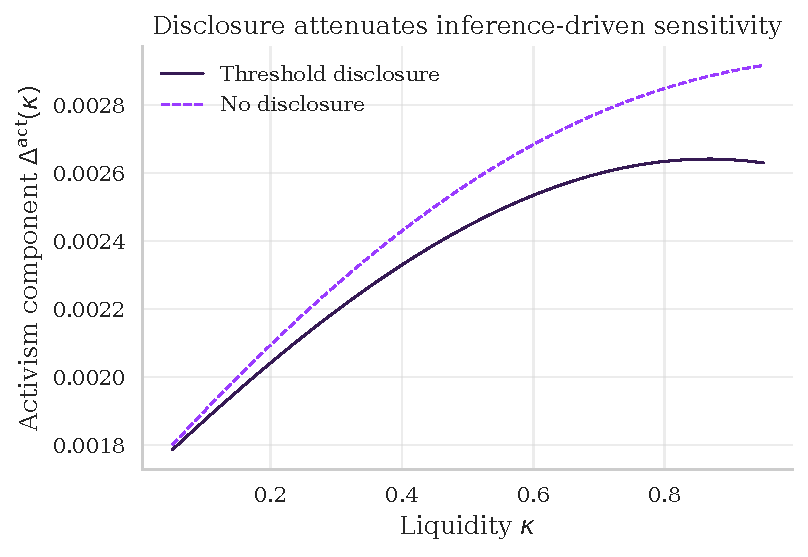
\includegraphics[height=0.65\textheight]{fig_disclosure.pdf}

\column{0.40\textwidth}
\textbf{$\obs{D}=1$ states:}
\begin{itemize}\itemsep0.1em
  \item $\outcome{\pi}(X,1) = 1$ always
  \item Expected premium $= \tilde{m}$
  \item Independent of $\kappa$
\end{itemize}

\vspace{0.4em}

\textbf{Sensitivity comes only from $\obs{D}=0$ states} where $\outcome{\pi}(X,0)$ varies with noise level.

\vspace{0.4em}

\textbf{Implication:}\\
Disclosure and liquidity are \textbf{substitutes} in shaping inference: more disclosure attenuates the non-monotone liquidity effect.
\end{columns}
\end{frame}

% ============================================================================
% IMPLICATIONS (Slides 15--17)
% ============================================================================

%Slide 15: Four Testable Predictions\begin{frame}{Four Testable Predictions}
\small
\begin{enumerate}\itemsep0.4em
  \item \textbf{Non-monotonic liquidity--premia:} Cross-sectionally, takeover premia should be hump-shaped in stock liquidity.\\
  {\footnotesize\textit{Test: quadratic liquidity term in premia regressions.}}

  \item \textbf{Disclosure moderates:} The liquidity--premia relationship should be stronger in non-disclosed settings and muted with clear disclosure.\\
  {\footnotesize\textit{Test: interact liquidity with 13D filing indicator.}}

  \item \textbf{Resistance wedge interaction:} Where activism increases resistance, disclosure should deter bids more sharply.\\
  {\footnotesize\textit{Test: triple interaction with activism type.}}

  \item \textbf{Inference vs observability:} Activist returns should be more sensitive to market conditions in quiet campaigns than in 13D-filing campaigns.\\
  {\footnotesize\textit{Test: compare returns in 13D vs non-13D activist positions.}}
\end{enumerate}
\end{frame}

%Slide 16: Policy Implications\begin{frame}{Policy: Liquidity Regulation as Governance Policy}
\small
\begin{columns}[T,onlytextwidth]
\column{0.55\textwidth}
\textbf{Disclosure threshold design:}
\begin{itemize}\itemsep0.1em
  \item Lower threshold $\Rightarrow$ more $D=1$ states
  \item More observability $\Rightarrow$ less inference-driven premia
  \item Tradeoff: transparency vs.\ activist incentives
\end{itemize}

\vspace{0.2em}

\textbf{Liquidity policy:}
\begin{itemize}\itemsep0.1em
  \item Liquidity regulation affects corporate control, not just trading costs
  \item Shapes the information environment for bidder entry
  \item Optimal liquidity may be interior (not maximal)
\end{itemize}

\column{0.43\textwidth}
\begin{block}{Key Takeaway}
Disclosure and liquidity policies are \textbf{substitutes} in shaping inference about engagement.

\vspace{0.2em}

The SEC 13D filing window debate should account for effects on takeover premia, not just trading profits.
\end{block}
\end{columns}
\end{frame}

%Slide 17: Summary\begin{frame}{Summary}
\footnotesize

\textbf{\textcolor{brightblue}{Mechanism}}\\[-0.2em]
{\usebeamercolor[fg]{block title}\rule{\linewidth}{0.4pt}}\\[0.2em]
Liquidity changes what order flow reveals about hidden engagement.
Disclosure creates observability vs.\ inference regimes.
Bidder entry depends on inferred engagement through the premium wedge.

\vspace{0.4em}

\textbf{\textcolor{brightblue}{Main Prediction}}\\[-0.2em]
{\usebeamercolor[fg]{block title}\rule{\linewidth}{0.4pt}}\\[0.2em]
Minority takeover gains are \textbf{hump-shaped} in liquidity:
bid incidence rises but the activism premium composition shifts.

\vspace{0.4em}

\textbf{\textcolor{brightblue}{Contribution}}\\[-0.2em]
{\usebeamercolor[fg]{block title}\rule{\linewidth}{0.4pt}}\\[0.2em]
Unifies exit/voice, informed trading, and takeover literatures through an inference-based mechanism.

\vspace{0.6em}
\centering
\textbf{Thank you!}\\[0.2em]
\texttt{austin.li@ucl.ac.uk}
\end{frame}

% ============================================================================
% REFERENCES
% ============================================================================

\begin{frame}[allowframebreaks]{References}
\small
\printbibliography
\end{frame}

% ============================================================================
% BACKUP SLIDES
% ============================================================================

\appendix

%Backup B1: Notation Guide\begin{frame}{Backup: Notation Guide}
\small
\begin{columns}[T,onlytextwidth]
\column{0.48\textwidth}
\begin{tabular}{@{}ll@{}}
\toprule
\multicolumn{2}{l}{\textbf{\choice{Choices / Actions}}} \\
\midrule
$\choice{q} \in \{-1,0,+1\}$ & Trade decision \\
$\choice{a} \in \{0,1\}$ & Engagement decision \\
$\choice{z} \in \{-1,0,+1\}$ & Noise trade \\
\midrule
\multicolumn{2}{l}{\textbf{\obs{Observables / Information}}} \\
\midrule
$\obs{X} = q + z$ & Order flow \\
$\obs{D} = \1\{q=+1\}$ & Disclosure flag \\
$\obs{s}$ & Private signal \\
$\obs{v}$ & Fundamental value \\
\bottomrule
\end{tabular}

\column{0.48\textwidth}
\scriptsize
\begin{tabular}{@{}ll@{}}
\toprule
\multicolumn{2}{l}{\textbf{\outcome{Equilibrium Outcomes}}} \\
\midrule
$\outcome{P}(X,D)$ & Price \\
$\outcome{\pi}(X,D)$ & Posterior engagement prob. \\
$\outcome{p}(P,D)$ & Bid probability \\
$\outcome{m}(X,D)$ & Expected premium \\
\midrule
\multicolumn{2}{l}{\textbf{Parameters}} \\
\midrule
$\kappa$ & Liquidity (noise prob.) \\
$k_1, k_0, k_D$ & Signal cutoffs \\
$\rho$ & Success prob. \\
$m_0, m_1$ & Base / success premium \\
$\tilde{m}$ & Expected premium \\
$\Delta, \tilde{\Delta}$ & Value-add; $\tilde{\Delta}=\rho\Delta$ \\
\bottomrule
\end{tabular}
\end{columns}

\vspace{0.4em}
\centering
{\footnotesize \textbf{Color coding:} \choice{Blue} = choices/actions \quad \obs{Red} = observables \quad \outcome{Green} = outcomes}
\end{frame}

%Backup B2: Baseline Calibration\begin{frame}{Backup: Baseline Calibration}
\begin{columns}[T,onlytextwidth]
\column{0.42\textwidth}
\scriptsize
\begin{table}
\centering
\setlength{\tabcolsep}{3pt}
\renewcommand{\arraystretch}{1.05}
\begin{tabular}{l r}
\toprule
\multicolumn{2}{l}{\textbf{Baseline calibration}}\\
\midrule
Discount factor $\delta$ & 0.95\\
Liquidity $\kappa$ & 0.50\\
Engagement: $(C_0, \chi)$ & (0.12, 0.50)\\
Engagement: $(\Delta, \rho)$ & (0.25, 0.90)\\
Resistance: $(m_0, m_1)$ & (0.10, 0.30)\\
Baseline synergy $\bar{S}$ & 1.44\\
Entry cost / shock $(K, \sigma_\xi)$ & (0.15, 0.40)\\
Signal noise $(\sigma_v, \sigma_\varepsilon)$ & (0.50, 0.50)\\
\bottomrule
\end{tabular}
\end{table}

\vspace{0.2em}
\footnotesize Cutoffs: $k_1 = k_0 \approx 0.82$, $k_D \approx 2.26$.

\column{0.58\textwidth}
\scriptsize
\begin{table}
\centering
\setlength{\tabcolsep}{3pt}
\renewcommand{\arraystretch}{1.05}
\resizebox{\linewidth}{!}{\begin{tabular}{llrrrr}
\toprule
$D$ & Order flow $X$ & $P(X,D)$ & $\pi(X,D)$ & $p(X,D)$ & $m(X,D)$ \\
\midrule
0 & $-2$ & 0.84 & 0.00 & 0.81 & 0.10 \\
0 & $-1$ & 1.06 & 0.41 & 0.55 & 0.17 \\
0 & $0$ & 1.23 & 0.74 & 0.33 & 0.23 \\
0 & $1$ & 1.39 & 1.00 & 0.17 & 0.28 \\
\midrule
1 & $0$ & 1.90 & 1.00 & 0.01 & 0.28 \\
1 & $1$ & 1.90 & 1.00 & 0.01 & 0.28 \\
1 & $2$ & 1.90 & 1.00 & 0.01 & 0.28 \\
\bottomrule
\end{tabular}
}
\end{table}

\vspace{0.2em}
\footnotesize
\begin{itemize}
  \item Disclosed states ($D=1$): $\pi = 1$, nearly flat prices
  \item Bids are rarer when $D=1$ due to higher resistance wedge
\end{itemize}
\end{columns}
\end{frame}

%Backup B3: Full Posterior Formulas\begin{frame}{Backup: Full Posterior Formulas}
\scriptsize
\textbf{With stake disclosure $D = \1\{q = +1\}$:}

\vspace{0.1em}

\begin{columns}[T,onlytextwidth]
\column{0.48\textwidth}
\textbf{Disclosed branch ($\obs{D}=1$):}
\begin{itemize}\itemsep0.1em
  \item $X \in \{0, 1, 2\}$ (since $q = +1$)
  \item $\pi(X, 1) = 1$ for all $X$
  \item Engagement fully observed
\end{itemize}

\column{0.48\textwidth}
\textbf{Non-disclosed branch ($\obs{D}=0$):}
\begin{itemize}\itemsep0.1em
  \item $X \in \{-2, -1, 0, 1\}$ (since $q \in \{-1, 0\}$)
  \item $\pi(X, 0)$ via Bayes' rule
  \item Depends on $\kappa$ through $(p_0, p_1)$
\end{itemize}
\end{columns}

\vspace{0.1em}

Let $p_0 = 1 - \kappa$, $p_1 = \kappa/2$:

\vspace{0em}

\begin{align*}
\outcome{\pi}(1,0) &= \frac{\omega_Q}{\omega_H + \omega_Q}\\[0.3em]
\outcome{\pi}(0,0) &= \frac{\omega_Q p_0}{(\omega_H + \omega_Q) p_0 + \omega_E p_1}\\[0.3em]
\outcome{\pi}(-1,0) &= \frac{\omega_Q p_1}{(\omega_H + \omega_Q) p_1 + \omega_E p_0}
\end{align*}

\vspace{0em}

\textbf{Note:} $\pi(1, 0) = \omega_Q / (\omega_H + \omega_Q)$ does \emph{not} depend on $\kappa$ because $X = 1$ with $D = 0$ pins down $q = 0$.
\end{frame}

%Backup B4: Pricing Fixed Point\begin{frame}{Backup: Solving the Pricing Fixed Point}
\small
For each information set $(X, D)$:

\begin{enumerate}
  \item Compute $\pi(X, D)$ from Bayes' rule
  \item Compute $\hat{V}(X, D) = \E[v \mid X, D] + \tilde{\Delta}\,\pi(X, D)$
  \item Solve scalar fixed point:
  \[
  P = \delta\big((1 - p(P, D))\,\hat{V} + p(P, D)(P + m(X, D))\big)
  \]
  where $p(P, D) = 1 - \Phi\left(\frac{m(X, D) + K - \bar{S} + P}{\sigma_\xi}\right)$

  {\scriptsize (We write $m(X,D)$ since $P(\cdot,D)$ is injective, so the bidder infers $X$ from $P$.)}
  \item Under the regularity condition (moderate feedback), the map is a contraction; iterate to convergence
\end{enumerate}

\vspace{0.3em}

\textbf{Regularity condition:} The derivative of bid probability w.r.t.\ price is bounded, ensuring a unique fixed point. Specifically, $\delta\,\phi(0)/\sigma_\xi < 1$.
\end{frame}

%Backup B5: Cutoffs vs Liquidity\begin{frame}{Backup: Cutoffs vs Liquidity}
\centering

\includegraphics[height=0.62\textheight]{fig_cutoffs_kappa.pdf}

\vspace{0.2em}
\footnotesize
\begin{itemize}\itemsep0pt
  \item Liquidity shifts Exit/Voice boundaries
  \item Weak ordering $k_1 \le k_0 \le k_D$ permits region collapse
  \item Exit becomes more attractive as $\kappa$ rises (noise cover for selling)
\end{itemize}
\end{frame}

%Backup B6: Price Function\begin{frame}{Backup: Price Function}
\centering

\includegraphics[height=0.62\textheight]{fig_prices.pdf}

\vspace{0.2em}
\footnotesize
\begin{columns}[T,onlytextwidth]
\column{0.48\textwidth}
\textbf{$D=0$ (non-disclosed):} Prices vary with $X$ as the market infers engagement probability from order flow.

\column{0.48\textwidth}
\textbf{$D=1$ (disclosed):} Prices are high and nearly flat across $X$; $\pi = 1$ ensures full activism premium.
\end{columns}
\end{frame}

%Backup B7: Sensitivity Analysis\begin{frame}{Backup: Sensitivity Analysis}
\small
\begin{columns}[T,onlytextwidth]
\column{0.50\textwidth}
\centering

\includegraphics[width=0.88\linewidth]{fig_sensitivity_C0.pdf}

{\footnotesize Varying engagement cost $C_0$}

\vspace{0.3em}
\footnotesize Higher $C_0$: shrinks voice regions, lowers activism premia, but can raise bids by lowering resistance expectations.

\column{0.50\textwidth}
\centering

\includegraphics[width=0.88\linewidth]{fig_sensitivity_wedge.pdf}

{\footnotesize Varying resistance wedge $m_1 - m_0$}

\vspace{0.3em}
\footnotesize Larger wedge: raises premia conditional on bid but deters entry through higher expected resistance.
\end{columns}
\end{frame}

%Backup B8: Alternative Disclosure Regimes\begin{frame}{Backup: Alternative Disclosure Regimes (FI / ND / NR)}
\footnotesize
Replace $(X, D)$ by $(X, S)$ with public signal $S$; define $\pi(X, S) = \PP(a = 1 \mid X, S)$.

\vspace{0.3em}

\begin{itemize}
  \item \textbf{FI (Full Information):} $S_{\text{FI}} = (q, a)$ reveals action $\Rightarrow$ inference channel shut down
  \item \textbf{ND (No Disclosure):} $S_{\text{ND}} = \emptyset$ $\Rightarrow$ engagement inferred from $X$ in \emph{all} states
  \item \textbf{NR (Noisy Rumor):} $S_{\text{NR}} = (D, R)$ adds a rumor $R$ informative about quiet engagement when $D = 0$
\end{itemize}

\vspace{0.3em}

\begin{center}
\scriptsize
\setlength{\tabcolsep}{3pt}
\renewcommand{\arraystretch}{1.05}
\resizebox{0.95\linewidth}{!}{%
  \begin{minipage}{\linewidth}
    \centering
    \begin{tabular}{lrrrr}
\toprule
$X$ & $\pi(X,0)$ & $\pi_{\textup{ND}}(X)$ & $\pi_{\textup{NR}}(X,0,R=0)$ & $\pi_{\textup{NR}}(X,0,R=1)$ \\
\midrule
$-1$ & 0.41 & 0.41 & 0.19 & 0.68 \\
$0$ & 0.74 & 0.74 & 0.48 & 0.89 \\
$1$ & 1.00 & 1.00 & 1.00 & 1.00 \\
\bottomrule
\end{tabular}
\vspace{0.6em}
\begin{tabular}{ll}
\toprule
$(q,a)$ & $\pi_{\textup{FI}}$ \\
\midrule
$(-1,0)$ & 0.00 \\
$(0,0)$ & 0.00 \\
$(0,1)$ & 1.00 \\
$(1,1)$ & 1.00 \\
\bottomrule
\end{tabular}

  \end{minipage}}
\end{center}

\vspace{0.2em}
\footnotesize\textbf{Message:} Disclosure informativeness/timing reshapes $\pi(\cdot)$ and hence the liquidity--premia mapping.
\end{frame}

\end{document}

